%version of 02-27-19

\chapter{EXERCISES}
\label{ch:Exercises}


\section{Summation}


\subsection{Compute $\Delta_n$ and sum of squares}

\ignore{$\Delta_n = \sum_{i=1}^{n} i = \frac{n(n+1)}{2}$

Use the same technique of writing the same sum by extracting the first and the last element provides a nice example.

We loose since the coefficient of the $\Delta_n$ is the same after these manipulations, but we can manage if we compute the \textit{next} sum, that is sum of the squares.
\medskip

$\Delta_{n+1} = 1 + \sum_{i=1}^{n+1} i $

$\Delta_{n+1} = (\sum_{i=1}^{n} i) + \frac{(n+1)(n+2)}{2}$
}

\section{Tetrahedral numbers}

The sum of the $\Delta_n$ is denoted by $\Theta_n$ and it is called a tetrahedral numbers:

$\Theta_n =  \sum_{k=1}^{n} \Delta_k$.

%We can show that: $\Theta_n = \frac{n.(n+1).(n+2)}{6}$

A way to prove this expression is to consider three copies of $\Theta_n$ and organize them in order to obtain the expected result
(remember the way we established the closed formula for triangular numbers was based on $2$ copies
arranged in the right form).
The basic tetrahedral number is organized as a triangle (see Figure~\ref{fig:TetrahedralBasic}).
The proof is obtained by Fubini's principle by rotating this triangle as shows in Figure~\ref{fig:Tetrahedral}.

\begin{figure}[h]
\begin{center}
        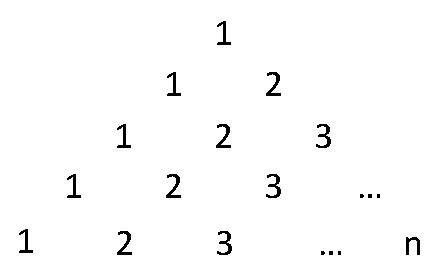
\includegraphics[scale=0.5]{FiguresArithmetic/TetrahedralBasic}
        \caption{Computing $\Theta_n$: basic triangle pattern.}
        \label{fig:TetrahedralBasic}
\end{center}
\end{figure}

The first row is equal to $n+2$.

The second one is equal to $3 + 2(n-1)+3 = 2(n+2)$. 

Let us sum up the elements in row $k$: 

$\Delta_k + k(n-k+1) + \Delta_k = k(k+1) +kn-k^2+k = k(n+2)$.

Thus, the global sum is equal to $n+2$ times $(1+2+...+n)$.

Finally, $3 \Theta_n = (n+2) \Delta_n$

\begin{figure}[h]
\begin{center}
        \includegraphics[scale=0.5]{FiguresArithmetic/Tetrahedral}
        \caption{Computing $\Theta_n$ using an adequate arrangement of $3$ triangles.}
        \label{fig:Tetrahedral}
\end{center}
\end{figure}

Summary and extension:

We proved some results, in particular:
\begin{itemize}
\item $Id_n = 1+1+ ... +1 = n$
\item $\Delta_n = 1+2+3+ ... +n = \frac{1}{2}.Id_n.(n+1)$
\item $\Theta_n = \Delta_1 + \Delta_2 + ... + \Delta_n = \frac{1}{3} .\Delta_n.(n+2)$
\end{itemize}

A natural question is if we can go further following the same pattern for computing $ \sum_{k=1}^{n} \Theta_k$, and so on.

\section{More exercises}

\subsection{Graphical proofs 1}

Compute sum of squares with 3 copies and fill the 2D rectangle. 
We should add here the figures that have been removed from the chapter SUMMATION. 
{\Denis put ref to the label here}

\subsection{Graphical proofs 2}

Computing the sum of $(\frac{1}{4})^k =\frac{1}{3} $ using a graphical argument.

The solution is depicted in Fig.~\ref{Fig:SUmgeo1sur4}. 
\begin{figure}
\begin{center}
        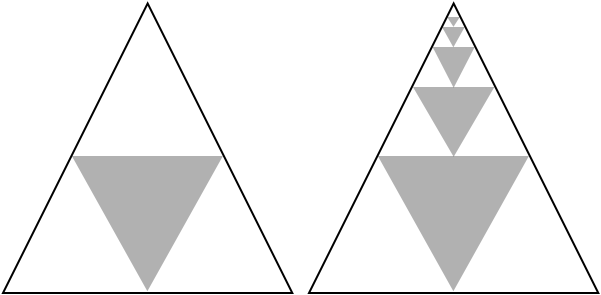
\includegraphics[scale=0.4]{FiguresArithmetic/SumGeometric1sur4}
        \caption{Graphical construction. Assuming the total surface is 1, the surface of the the internal triangle (in blue) is $\frac{1}{4}$.
        As the blue surface is one third at each layer, the global surface is $\frac{1}{3}$.
        By Fubini principle, this surface is the sum of the $\frac{1}{4^k}$ (for $k \geq 1$).}
        \label{Fig:SUmgeo1sur4}
\end{center}
\end{figure}


\subsection{Harmonic series}

$H_{n} = \sum_{k=1}^{n} \frac{1}{k}$.

Another way to prove that the sum is infinite:
 
The analysis is as follows.
Group the terms according to powers of $2$. 
The sum within each group is between $\frac{1}{2}$ and $1$, thus,
$H_n > \frac{1}{2}.n$
\\

Another (more precise) way is to gather the terms 3 by 3 as follows:

$S_k = (\frac{1}{3k-1} + \frac{1}{3k} + \frac{1}{3k+1} )$ for $k\geq1$, 

$H = 1 + S_1 + ... + S_k + ... > 1 + 3.\frac{1}{3} + 3.\frac{1}{6} + ... + 3.\frac{1}{3k} + ... $

since $S_k > 3.\frac{1}{k} $.

The proof is by contradiction, if $H$ is finite, from the previous relation we have: $H > 1 + H$, which is obviously impossible.
\bigskip

Moreover, the first way of  bounding the sum tells us about its value (actually, we know the value at a factor of $2$):

$\frac{log(n)+1}{2} < H_n < log(n)+1$. Thus, $H_n = O(log(n))$

{\Denis Change the writing of o}



\section{Arithmetic}

\subsection{A fun result: complex
  multiplication via $3$ real multiplications}
\index{complex number!multiplication via 3 real multiplications}

\begin{prop}
%\label{thm:complex-mult-3real}
One can compute the product of two complex numbers using {\em three}
real multiplications rather than four.
\end{prop}

\begin{proof}
Although implementing (\ref{eq:complex-mult}) ``directly'' correctly
produces the product $\kappa = (a+bi) \cdot (c+di)$, there is another
implementation that is {\em more efficient}.  Specifically, the
following recipe computes $\kappa$ using only {\em three} real
multiplications instead of the four real multiplications of the
``direct'' implementation.  We begin to search for this recipe by
noting that our immediate goal is to compute both Re$(\kappa) = ac-bd$
and Im$(\kappa) = ad+bc$.  We can accomplish this by computing the
{\em three} real products
\begin{equation}
\label{eq:complex-mult-3a}
(a+b) \cdot (c+d); \ \ \ \ \
ac;  \ \ \ \ \ bd
\end{equation}
and then noting that
\begin{equation}
\label{eq:complex-mult-3b}
\begin{array}{lcl}
\mbox{Im}(\kappa) & = & (a+b) \cdot (c+d) - ac -bd, \\
\mbox{Re}(\kappa) & = & ac -bd
\end{array}
\end{equation}
We thereby achieve the result of the complex multiplication described
in (\ref{eq:complex-mult}) while using only {\em three} real
multiplications.

Of course, a full reckoning of the costs of the two implementations we
have discussed exposes the fact that the implementation that invokes
(\ref{eq:complex-mult-3a}) and (\ref{eq:complex-mult-3b}) uses {\em
  three} real additions rather than the {\em two} real additions of
the ``direct'' implementation.  But this entire exercise was
predicated on the observation that each real addition is much less
costly than a real multiplication, so trading one multiplication for
one addition is an unqualified ``win''.  \qed
\end{proof}

Extension of the same method: 

Notice that this technique is classical and it has been used in many other situations.
For instance while multiplying two integers in base 2 (see exercice~{Karatsuba}).




\subsection{A Fun Result: A ``Trick'' for Squaring Certain Integers}

Sometimes only basic knowledge is needed to craft amusing
``tricks''---we know that they are not really tricks at all!---that
are really rigorous applications of principles that we have learned.
Here is an ``old chestnut'' example that may inspire you to design
your own. 

If someone presents you with a number that has a numeral that ends in
$5$, then there is a simple way to square the number mentally.  For
instance, if someone says

\hspace{.25in}``$n = 25$''

\noindent
then you can instantly respond

\hspace{.25in}``$n^2 = 625$''

\noindent
If the challenge is

\hspace{.25in}``$n = 75$''

\noindent
then your response is

\hspace{.25in}``$n^2 = 5625$''

\noindent
Let's make this ``game'' mathematical.

\begin{prop}
\label{thm:75x65=4925}
Let $n$ be any number that has a $2$-digit decimal numeral of the form

\hspace{.25in}$\delta \ 5$ \ \ \ \ $(\delta \in \{ 0,1,2,3,4,5,6,7,8,9\})$.

\noindent
Then the square of $n$ is the integer

\hspace{.25in}$25 \ + \ \delta \cdot (\delta +1)$. 
\end{prop}

\begin{proof}
We can rewrite the premise of the proposition in the form
\[ n \ = \ 10 \cdot \delta + 5 \]
It is now easy to invoke Proposition~\ref{prop:(a+b)(c+d)} and the
distributive law to compute that

\[ n^2 \ = \ 100 \cdot \delta \cdot (\delta+1) + 25. \]
To wit: 
\[
\begin{array}{lclll}
n^2 & = & (10 \cdot \delta + 5)^2 & & \mbox{Given} \\
    & = & 100 \cdot \delta^2 \ + \ 100 \cdot delta \ + \ 25
              & & \mbox{the proposition} \\
    & = & 100 \cdot (\delta^2 \ + \ \delta) \ + \ 25
              & & \mbox{factoring: distributive law} \\
    & = & 100 \cdot \delta \cdot (\delta + 1) \ + \ 25
              & & \mbox{factoring: distributive law} \\
\end{array}
\]
A parlor trick has become a mathematical demonstration!
\qed
\end{proof}


\subsection{A fun result via geometric sums: When is integer  $n$
  divisible by $9$?}
\label{sec:divisible-by-9}

We now exploit our ability to evaluate geometric summations to
illustrate a somewhat surprising, nontrivial fact.  One can deduce
information about the divisibility of an integer $n$ from $n$'s
positional numerals.  We hope that this ``fun'' result will inspire
the reader to seek kindred numeral-encoded properties of numbers.

\begin{prop}
\label{thm:div-by-b-bar}
An integer $n$ is divisible by an integer $m$ if, and only if, $m$
divides the sum of the digits in the base-$(m+1)$ numeral for $n$.
\end{prop}

The most familiar instance of this result is phrased in terms of our
traditional use of base-$10$ (decimal) numerals. \\
{\it An integer $n$ is divisible by $9$ if, and only if, the sum of
  the digits of $n$'s base-$10$ numeral is divisible by $9$.}

\smallskip

\begin{proof}
({\it Argument for general number-base $b$}).
%
Of course, we lose no generality by focusing on numerals without
leading $0$'s, because leading $0$'s do not alter a numeral's sum of
digits.

Let us focus on the base-$b$ numeral for a number $n$ (so $b = m+1$ in
the statement of the proposition).  There therefore exist base-$b$
digits---i.e., integers from the set $\{0, 1, \ldots, b-1\}$---call
them $\delta_k \neq 0$, $\delta_{k-1}$, \ldots $\delta_1$, $\delta_0$,
such that
\[ n \ = \ \delta_k \cdot b^k + \delta_{k-1} \cdot b_{k-1} + \cdots +
\delta_1 \cdot b + \delta_0. \]
The sum of the digits of $n$'s base-$b$ numeral is, then
\[ s_b(n) \ \eqdef \ \delta_k + \delta_{k-1} + \cdots + \delta_1 +
\delta_0. \]
Let us calculate the difference $n - s_b(n)$ in the following manner,
digit by digit.
\begin{equation}
\label{eq:sum-of-digits}
\begin{array}{ccccccccccc}
n & = &
\delta_k \cdot b^k & + & \delta_{k-1} \cdot b^{k-1} & + & \cdots
  & + & \delta_1 \cdot b & + & \delta_0 \\
s_b(n) & = &
\delta_k & + & \delta_{k-1} & + & \cdots & + & \delta_1 & + & \delta_0 \\
\hline
n - s_b(n) & = &
\delta_k \cdot (b^k -1) & + &
\delta_{k-1} \cdot (b^{k-1} -1) & + &
\cdots & + &
\delta_1 \cdot (b-1) & & 
\end{array}
\end{equation}

\medskip

We now revisit summation (\ref{eq:geom-sum:b>1}).  Because $b$ is a
positive integer, so that $1 + b + \cdots + b^{a-2} + b^{a-1}$ is also
a positive integer, we infer that {\em the integer $b^a -1$ is
  divisible by $b-1$.}

We are almost home.  Look at the equation for $n - s_b(n)$ in the
system (\ref{eq:sum-of-digits}).  As we have just seen, every term on
the righthand side of that equation is divisible by $b-1$.  It follows
therefore, that the lefthand expression, $n - s_b(n)$, is also
divisible by $b-1$.
An easy calculation, which we leave to the reader, now shows that this
final fact means that $n$ is divisible by $b-1$ if, and only if,
$s_b(n)$ is.
\end{proof}



%%%%%%%%%%%%%%%%%%%%%%%%%%%%%%%%%%%%%

\section{Pairing Functions as Encodings of $\N^+ \times \N^+$ as $\N^+$}
\label{Appendix:building-pairing-functions}

{\Denis The introduction has been taken from the main part of the book,
it has to be rewritten}

The remainder of this section is devoted to developing {\em easily
  computed} bijections between the set $\N^+ \times \N^+$ and the set
$\N^+$ of positive integers.  We thereby exhibit easily computed
mechanisms for \underline{encoding} ordered pairs of integers---hence,
also, tuples, strings, and binary trees of integers---as single
integers.  We thereby see that---at least within the world of integers
and entities encodable as integers---there is no intrinsic new power
inherent in tuple-spaces: \index{tuple-spaces} {\em Sets of tuples of
  integers can be effiiciently encoded as sets of integers.}  Because
of the special role of ordered pairs of integers in our study of
encodings of structured sets of integers---they form the fundamental
puzzle from whose solution all else will follow---a special name has
been associated with bijections between $\N^+ \times \N^+$ and $\N^+$.
These special bijections are called {\it pairing functions}.
\index{pairing functions!encodings}

One of the most valuable by-products of encodings provided by pairing
functions is that such encodings provide {\em linear orderings} of the
\index{pairing functions!linear orderings}
set being encoded.  We noted in Section~\ref{sec:integers}.A that
``order within a number system is among one's biggest friends when
reasoning about the numbers within the system.''  The orderings
provided by these encodings are particularly
valuable when the structured sets being encoded as integers do not
have their own ``intrinsic'' or ``natural'' orderings.  Included in
this category are  structures such as tuples,
strings, and trees.
\bigskip

\ignore{\noindent \fbox{
\begin{minipage}{0.95\textwidth}
Of course some structured sets do have natural, native linear orders:
consider, as one such, strings under lexicographic ordering.  Even for
such sets, we often benefit from having alternative orderings as we
design and analyze algorithms on the sets.
\end{minipage}
}
\bigskip
}

We focus on $\N^+$ as the avatar of {\it integer}, rather than on $\Z$
or $\N$, primarily for definiteness and a bit of clerical
simplification.  We could easily rewrite this section with a focus on
bijections between $\Z \times \Z$ and $\Z$ or on bijections between
$\N \times \N$ and $\N$.

\bigskip

We now embark on a very short guided tour that will introduce the
reader to three interesting pairing functions.  The reader should note
that the diagonal pairing function of Section~\ref{sec:diag-pair-fn}
and the square-shell pairing function of
Section~\ref{sec:square-pair-fn} build in essential ways on the
$L$-norms of Section~\ref{sec:Ln-norms}; cf., Fig.~\ref{fig:Ln-discs}.

\subsection{The Diagonal pairing function $\d$}
\label{sec:diag-pair-fn}
\index{The Diagonal pairing function $\d$}

Pairing functions first appeared in the literature early in the 19th
century.  Perhaps the simplest and ``prettiest'' such function (since
it is a {\em polynomial}) appears, pictorially, in an 1821 work by the
great French mathematician Augustin Cauchy \cite{Cauchy21}.
\index{Cauchy, Augustin}
%
This {\em diagonal} pairing function was formally specified a
half-century later by the German logician Georg Cantor,
\index{Cantor, Georg}
%
whose studies \cite{Cantor74,Cantor78} revolutionized how we think
about {\em infinite} sets.

\begin{equation}
\label{eq:diag}
\d(x, y) \ = \
{{x+y-1} \choose 2} + (1-y)
\end{equation}
($\d$ of course has a twin that exchanges $x$ and $y$).  $\d$'s
mapping of $\N^+ \times \N^+$ onto $\N^+$, as depicted in
Fig.~\ref{fig:diag}, exposes that we can view $\d$'s mapping of $\N^+
\times \N^+$ as a two-step conceptual process:
\begin{figure}[htb]
\begin{center}
      \includegraphics[scale=0.4]{FiguresArithmetic/PairingDiagonal}
%\begin{tabular}{r|r|r|r|r|r|r|r|r}
% 1 &  3 &  6 & 10 & \fbox{15} &  21 &  28 &  36 & $\cdots$ \\
% 2 &  5 &  9 & \fbox{14} & 20 &  27 &  35 &  44 & $\cdots$ \\
% 4 &  8 & \fbox{13} & 19 & 26 &  34 &  43 &  53 & $\cdots$ \\
% 7 & \fbox{12} & 18 & 25 & 33 &  42 &  52 &  63 & $\cdots$ \\
%\fbox{11} & 17 & 24 & 32 & 41 &  51 &  62 &  74 & $\cdots$ \\
%16 & 23 & 31 & 40 & 50 &  61 &  73 &  86 & $\cdots$ \\
%22 & 30 & 39 & 49 & 60 &  72 &  85 &  99 & $\cdots$ \\
%29 & 38 & 48 & 59 & 71 &  84 &  98 & 113 & $\cdots$ \\
%$\vdots$ & $\vdots$ & $\vdots$ & $\vdots$ & $\vdots$ & $\vdots$ &
%  $\vdots$ & $\vdots$ & $\ddots$
%\end{tabular}
\end{center}
\caption{{\it The diagonal pairing function $\d$.  The shell $x+y = 6$
    is highlighted.}
\label{fig:diag}}
\end{figure}
\begin{enumerate}
\item
partitioning $\N^+ \times \N^+$ into ``diagonal shells'' defined as
\[
\{ \langle x,y \rangle \ | \ x+y = 2 \}, \ \ 
\{ \langle x,y \rangle \ | \ x+y = 3 \}, \ \ 
\{ \langle x,y \rangle \ | \ x+y = 4 \}, \ \ \ldots
\]
This is accomplished by the following subexpression in (\ref{eq:diag}).
\[
{1 \over 2} (x+y) \cdot (x+y-1) \ = \ {{x+y-1} \choose 2}
\]

\item
``climbing up'' these shells in order.

This is accomplished by the additional subexpression ``$+1-y$'' in
(\ref{eq:diag}).
\end{enumerate}
\bigskip

\noindent \fbox{
\begin{minipage}{0.95\textwidth}
%\[ \approx \approx \approx \approx \approx \approx \approx \approx \approx \approx \]
Keep in mind that we have just described a {\em conceptual}
  process.  $\d$ is a function, {\em not} an algorithm.  ``Running''
  this infinite process would take forever.
%\[ \approx \approx \approx \approx \approx \approx \approx \approx \approx \approx \]
\end{minipage}
}
\bigskip

Understanding $\d$'s structure leads to a broadly applicable strategy
for inductively constructing a broad range of pairing functions.  We
develop this strategy in Subsection B, along with an accompanying
rather simple inductive verification of bijectiveness.  One finds a
computationally more satisfying proof of $\d$'s bijectiveness in
\cite{Davis58}, along with an explicit recipe for computing $\d$'s
inverse.  The material in \cite{Davis58} builds specifically on $\d$'s
structure.
\bigskip

\noindent \fbox{
\begin{minipage}{0.95\textwidth}
%\[ \approx \approx \approx \approx \approx \approx \approx \approx \approx \approx \]
{\small\sf $\oplus$ Esoterica for enrichment:}
The fact that $\d$ is a {\em polynomial} in $x$ and $y$ raises
  the natural (to a mathematician!)~question of whether there exist
  any other polynomial pairing functions.  This is a quite advanced
  topic that is beyond the scope of this text.  Indeed, even as a
  research problem, the question remains largely open.  But, a few
  nontrivial pieces of an answer are known.
\begin{enumerate}
\item
There is no {\em quadratic} polynomial pairing function other than
$\d$ (and its twin) \cite{FueterP23,LewR78a}.
\item
No {\em cubic} or {\em quartic} polynomial is a pairing function
\cite{LewR78b}.
\item
The development in \cite{LewR78b} excludes large families of
higher-degree polynomials from being pairing functions; e.g., a {\em
  super-quadratic} polynomial whose coefficients are all positive
cannot be a pairing function.
\end{enumerate}
\end{minipage}
}
%\[ \approx \approx \approx \approx \approx \approx \approx \approx \approx \approx \]

\subsection{A methodology for crafting pairing functions}
\label{sec:build-pair-fn}
\index{constructing pairing functions via ``shells''}
\index{pairing functions as storage mappings for arrays/tables}

The shell-oriented strategy that underlies the diagonal pairing
function $\d$ can be adapted to incorporate shell-``shapes'' that are
inspired by a variety of computational situations---and can be applied
to great computational advantage in such situations.  We describe how
such adaptation can be effected, and we describe a few explicit shapes
and situations.  We invite the reader to craft others.

\medskip

{\Denis Change the style for writing the algorithms -- We should guarantee the coherency all over the book!}

\noindent {\underline{\bf Procedure}} {\small\sf PF-Constructor}($\a$) \\
/*Construct a shape-inspired pairing function (PF) $\a$*/
\begin{description}
\item[Step 1.]
%
Partition the set $\N^+ \times \N^+$ into finite sets called {\it
  shells}.  Order the shells linearly in some way: many natural
shell-partitions carry a natural order.
\end{description}
As noted above, Shell $c$ of the diagonal pairing function $\d$ is the
following subset of $\N^+ \times \N^+$: $\{ \langle x,y \rangle \ |
\ x+y = c \}$.  The parameter $c$ orders $\d$'s shells.

\begin{description}
\item[Step 2.]
Construct a pairing function from the shells as follows.
  \begin{description}
  \item[Step 2a.]
Enumerate $\N^+ \times \N^+$ shell by shell, honoring the ordering of
the shells; i.e., list the pairs in shell \#1, then shell \#2, then
shell \#3, etc.
  \item[Step 2b.]
Enumerate each shell in some systematic way, e.g., ``by columns'':
Enumerate the pairs $\langle x,y \rangle$ in each shell in increasing
order of $y$ and, for pairs having equal $y$ values, in decreasing
order of $x$.
  \end{description}
\end{description}

\begin{prop}
\label{thm:PF-construct}
Any function $\a: \N^+ \times \N^+ \leftrightarrow \N^+$ that is
designed via Procedure {\small\sf PF-Constructor} is a bijection.
\end{prop}

\begin{proof}(Sketch) Step 1 of Procedure {\small\sf PF-Constructor}
constructs a partial order on $\N^+ \times \N^+$, in which: ($a$) each
shell is finite; ($b$) there is a linear order on the shells.  Step 2
extends this partial order to a linear order, by honoring the inherent
ordering of shells and imposing a linear order within each shell.  The
function constructed via the Procedure is: {\em injective} because the
disjoint shells are enumerated sequentially; {\em surjective} because
the enumeration within each shell begins immediately after the
enumeration within the preceding shell, with no gap.  \qed
\end{proof}

\bigskip

We have noted how to use Procedure {\small\sf PF-Constructor} to
construct pairing function $\d$.  We now use the Procedure to design
two other useful pairing functions.

\subsection{The Square-shell pairing function $\s$}
\label{sec:square-pair-fn}
\index{The Square-shell pairing function $\s$}

One computational situation where pairing functions can be useful
involves storage-mappings for arrays/tables that can expand and/or
contract dynamically.  In conventional systems, when one expands an $n
\times n$ table into an $(n+1) \times (n+1)$ table, one allocates a
new region of $(n+1)^2$ storage locations and copies the current table
from its $n^2$-location region to the new region.  Of course, this is
very wasteful: one is moving $\Omega(n^2)$ items to make room for the
anticipated $2n+1$ new items.  On any given day, the practical impact
of this waste depends on current technology.  But, this is a
mathematics text, not an engineering one, so we are exploring whether
{\em in principle} we can avoid the waste.  The answer is ``YES''.  If
we employ a pairing function $\varepsilon: \N^+ \times \N^+
\leftrightarrow \N^+$ to allocate storage for tables, then to expand a
table from dimensions $n \times n$ to $(n+1) \times (n+1)$, we need
move only $O(n)$ items to accommodate the {\em new} table entries; the
current entries need not be moved.  For square tables, the following
{\it Square-shell} pairing function $\s$ manages the described
scenario perfectly.  After describing $\s$, we comment on managing
tables of other shapes.
\begin{figure}[htb]
\begin{center}
%\begin{tabular}{r|r|r|r|r|r|r|r|r}
%  1 &  4 &  9 & 16 & \fbox{25} &  36 &  49 &  64 & $\cdots$ \\
%  2 &  3 &  8 & 15 & \fbox{24} &  35 &  48 &  63 & $\cdots$ \\
%  5 &  6 &  7 & 14 & \fbox{23} &  34 &  47 &  62 & $\cdots$ \\
% 10 & 11 & 12 & 13 & \fbox{22} &  33 &  46 &  61 & $\cdots$ \\
%\fbox{17} & \fbox{18} & \fbox{19} & \fbox{20} & \fbox{21} &  32 &  45
%  &  60 & $\cdots$ \\ 
% 26 & 27 & 28 & 29 & 30 &  31 &  44 &  59 & $\cdots$ \\
% 37 & 38 & 39 & 40 & 41 &  42 &  43 &  58 & $\cdots$ \\
% 50 & 51 & 52 & 53 & 54 &  55 &  56 &  57 & $\cdots$ \\
%$\vdots$ & $\vdots$ & $\vdots$ & $\vdots$ & $\vdots$ & $\vdots$ &
%  $\vdots$ & $\vdots$ & $\ddots$
%\end{tabular}
   \includegraphics[scale=0.4]{FiguresArithmetic/PairingSquareShell}
\end{center}
\caption{{\it The square-shell pairing function $\s$.  The shell
    $\max(x,y) = 5$ is highlighted.}
\label{fig:pairingSquareShell}}
\end{figure}
\begin{equation}
\label{e.square}
\begin{array}{ccl}
\s(x, y) & = & m^2 + m + y-x+1 \\
 & & \mbox{where } \ \ \  m \ \eqdef \ \max(x-1,y-1).
\end{array}
\end{equation}
One sees in Fig.~\ref{fig:pairingSquareShell} that $\s$ follows the
prescription of Procedure PF-Constructor: (1) it maps integers into
the ``square shells'' defined by: $m = 0, \ m = 1, ...$.  (2) it
enumerates the entries in each shell in a counterclockwise direction.
(Of course, $\s$ has a twin that enumerates the shells in a clockwise
direction.)
\bigskip

\noindent \fbox{
\begin{minipage}{0.95\textwidth}
%\[ \approx \approx \approx \approx \approx \approx \approx \approx \approx \approx \]
Using somewhat more complicated instantiations of Procedure
  PF-Constructor, the study in \cite{Rosenberg75} adapts the
  square-shell pairing function $\s$ to: ($a$) accommodate, with no
  wastage, arrays/tables of any fixed aspect ratio $an \times bn$
  ($a,b \in \N$); ($b$) accommodate, with only $O(n)$ wastage,
  arrays/tables whose aspect ratios come from a fixed finite set of
  candidates---i.e., $(a_1 n \times b_1 n)$ or $(a_2 n \times b_2 n)$
  or \ldots or $(a_k n \times b_k n)$.
%\[ \approx \approx \approx \approx \approx \approx \approx \approx \approx \approx \]
\end{minipage}
}

\subsection{$\oplus$ The Hyperbolic-shell pairing function $\h$}
\label{Appendix:hyp-shell-pair-fn}
\index{The Hyperbolic-shell pairing function $\h$}

We have just seen, in subsections B and C, that when the growth
patterns of one's arrays/tables is very constrained, one can use
pairing functions as storage mappings with very little wastage.  In
contrast, if one employs a pairing function such as $\d$ without
consideration of its wastage, then a storage map would show some
$O(n)$-entry tables being ``spread'' over $\Omega(n^2)$ storage
locations.  In the worst-case, $\d$ spreads the $n$-position $1 \times
n$ array/table over $> {1 \over 2} n^2$ addresses: $\d(1,1) = 1$ and
$\d(1,n) = {1 \over 2} (n^2 + n)$.  This degree of wastefulness can be
avoided via careful analysis, coupled with the use of Procedure
PF-Constructor.  The target commodity to be minimized is the {\it
  spread} of a PF-based storage map, which we define as follows.
\index{the spread of a pairing function}

Note that an ordered pair of integers $\langle x,y \rangle$ appears as
a position-index within an $n$-position table if, and only if, $xy
\leq n$.  Therefore, we define the spread of a PF-based storage map
$\m$ via the function
\begin{equation}
\label{e.compact}
{\bf S}_{\cal M}(n) \ \eqdef \ \max\{ \m(x, y) \ | \ xy \leq n \}.
\end{equation}
${\bf S}_{\cal M}(n)$ is the largest ``address'' that PF $\m$ assigns
to any position of a table that has $n$ or fewer positions.

Happily, the tools we have developed enable us to design a pairing
function that (to within constant factors) has minimum worst-case
spread.  This is the {\em Hyperbolic-shell pairing function} $\h$ of
(\ref{e.hyper}) and Fig.~\ref{fig:pairingHyper}.\footnote{Details appear in
  \cite{Rosenberg74,Rosenberg75}.}
\begin{equation}
\label{e.hyper}
\begin{array}{lcll}
\multicolumn{4}{l}{\mbox{Let $\delta(k)$ be the number of divisors of
    the integer $k$.}} \\
\h(x,y) & = & {\displaystyle \sum_{k=1}^{xy-1} \delta(k) \ \ +} &
  \mbox{the position of } \ \langle x, y \rangle \ \mbox{ among 2-part} \\
        &   &  & \mbox{factorizations of the number $xy$, in} \\
        &   &  & \mbox{reverse lexicographic order}
\end{array}
\end{equation}
\begin{figure}[htb]
\begin{center}
%\begin{tabular}{r|r|r|r|r|r|r|r}
% 1 &  3 &  5 &   8 &  10 & \fbox{14} &  16  & $\cdots$ \\
% 2 &  7 & \fbox{13} &  19 &  26 &  34 &  40 & $\cdots$ \\
% 4 & \fbox{12} & 22 &  33 &  44 &  56 &  69 & $\cdots$ \\
% 6 & 18 & 32 &  48 &  64 &  81 &  99  & $\cdots$ \\
% 9 & 25 & 43 &  63 &  86 & 108 & 130  & $\cdots$ \\
%\fbox{11} & 31 & 55 &  80 & 107 & 136 & 165 & $\cdots$ \\
%15 & 39 & 68 &  98 & 129 & 164 & 200  & $\cdots$ \\
%17 & 47 & 79 & 116 & 154 & 193 & 235  & $\cdots$ \\
%$\vdots$ & $\vdots$ & $\vdots$  & $\vdots$ & $\vdots$ &
%  $\vdots$ & $\vdots$ & $\ddots$
%\end{tabular}
      \includegraphics[scale=0.4]{FiguresArithmetic/PairingHyper}
\end{center}
\caption{{\it The hyperbolic pairing function $\h$.  The shell $xy = 6$ is
highlighted.}
\label{fig:pairingHyper}}
\end{figure}


\begin{prop}[\cite{Rosenberg75}]
\label{thm:hyp-opt}
{\bf (a)}
The hyperbolic function $\h$ is a pairing function.

\noindent {\bf (b)}
The spread of $\h$ is given by
${\bf S}_{\cal H}(n) \ = \ O(n \log n)$.\footnote{A  detailed
  analysis reveals that the spread of $\cal H$ is closely related to
  the {\em natural} logarithm, whose base is Euler's constant $e$.}

\noindent {\bf (c)}
No pairing function has better compactness than $\h$ (in the worst
case) by more than a constant factor.
\end{prop}

\begin{proof}
{\bf (a)} The fact that $\h$ is a pairing function follows from
Proposition~\ref{thm:PF-construct}.

\noindent {\bf (b)}
The pairing function $\h$ maps integers along the ``hyperbolic
shells'' defined by $xy = 1, \ xy =2, \ xy=3, \ldots$.  Hence,
when an integer $n$ is ``placed'' into the table of values of
$\h$, the number of occupied slots is within $n$ of
\[ \sum_{i=1}^{n-1} \ |\{ \langle x,y \rangle \ | \ xy < i \}| 
\]
Elementary calculations show that this sum is $O(n \log n)$.

\noindent {\bf (c)} The optimality of $\h$ in compactness (up to
constant factors) is seen via the following argument.  The set of
tables that have $n$ or fewer positions are those of aspect ratios
$a_i \times b_i$, where $a_i b_i \leq n$.  As one sees from
Fig.~\ref{f.hyp} (generalized to arbitrary $n$), the union of the
positions of all these arrays is the set of integer lattice points
under the hyperbola $xy = n$.  It is
well-known---cf.~\cite{NivenZ80}---that this set of points has
cardinality $\Theta(n \log n)$.\footnote{Recall from
  Chapter~\ref{sec:set-concepts} that the {\it cardinality} of a
  finite set $S$ is the number of elements in $S$.}  Since every table
contains position $\langle 1,1 \rangle$, it follows that, for every
$n$, some table containing $n$ or fewer positions is spread over
$\Omega(n \log n)$ ``addresses.''  \qed
\end{proof}
\begin{figure}[htb]
\begin{center}
       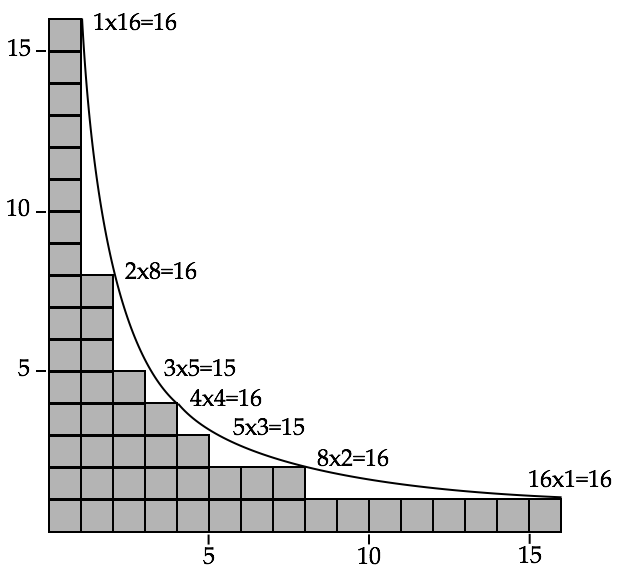
\includegraphics[scale=0.4]{FiguresArithmetic/PairingHyp}
\caption{The aggregate set of positions of tables having $16$ or
    fewer position.  To help the reader understand the figure, we
    include the curve $f(x,y) = xy$ which provides an upper envelope
    for the set.  A careful look at this curve will reveal that it
    touches the set of positions at the points $\langle x,y \rangle
    \in \{ \langle 1,16 \rangle, \ \langle 2,8 \rangle, \ \langle 4,4
    \rangle, \ \langle 8,2 \rangle, \ \langle 16,1 \rangle \}$, but it
    does {\em not} touch the set at the points $\langle x,y \rangle
    \in \{ \langle 3,5 \rangle, \ \langle 5,3 \rangle \}$. 
\label{f.hyp}}
\end{center}
\end{figure}

%%%%%%%%%%%%%%%%%%%%%%%%%%%%%%%%%%%%

\section{A System Based on the Fibonacci Numbers}
\label{sec:numerals-special-families}
\label{sec:Fibo-numbers}

{\Denis write a short introduction here}

In a variety of application areas, the special properties of certain
families of numbers can be exploited if one uses the numbers in the
family to devise representations of all integers.  We illustrate this
fact while using the Fibonacci numbers---see
Section~\ref{sec:Fibonacci}---as our basis family.

\noindent
We shall repeatedly find the following nonstandard notation useful:

For integers $m$ and $n$, we write $[m \gg n]$ to mean that $m \geq
n+2$.

\medskip


We will first prove the \textit{Zeckendorf's theorem} which states
that every positive integer $n$ has a unique representation of the
form:  **CITATION**

$n = F(k_1) + F(k_2) + ... + F(k_r)$ where $k_1 \gg k_2 \gg ... \gg k_r$ and $k_r \geq 2$.

Here, we assume that the Fibonacci sequence starts at index $1$ and not $0$,
moreover, the decompositions will never consider $F(1)$ (since $F(1)=F(2$)). 
For instance, the representation of $12345$ turns out to be:

$12345 = 10946 + 987 + 377 + 34 + 1 = F(21) + F(16) + F(14) + F(9) + F(2)$
\bigskip

Figure~\ref{zeckendorf} shows the decomposition of the first 26 integers written in this system. 
\begin{figure}[h]
\begin{center}
%\includegraphics[width=0.4\textwidth]{../FIGmaths/zeckendorf_representations.png}
        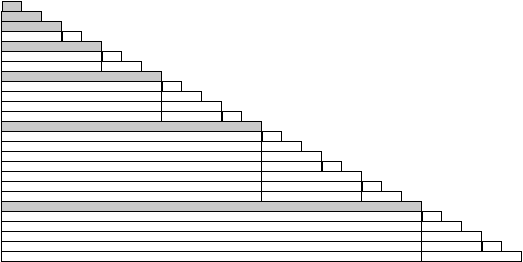
\includegraphics[scale=0.6]{FiguresArithmetic/Zeckendorf}
        \caption{The first integers (on the Y-axis) broken down into the Zeckendorf representation.
        The shaded rows corresponds to pure Fibonacci numbers.}
\label{zeckendorf}
\end{center}
\end{figure}

\noindent \textbf{Proof of Zeckendorf's Theorem}

The proof is done by induction on $n$ for proving simultaneously both construction and uniqueness.

\begin{itemize}
\item
The basis is true since the decomposition is obviously unique for $n=2$ (and also for $n=3$). 
Notice that for $n=4$, we have $4 = 3 + 1 = F(4) + F(2)$. 

\item
Assume for the induction step that any integer strictly lower than $F(k)$ can be decomposed uniquely as the sum of non-consecutive Fibonacci numbers.
We will prove as a consequence that an integer $n$ in the next interval between two consecutive Fibonacci numbers $F(k) \leq n < F(k+1)$ may be decomposed. 

If $n=F(k)$ is a Fibonacci number, the decomposition is reduced to $F(k)$.

Moreover, it is not difficult to check that it is unique.

%by using Property~\ref{prop:FiboSum}:
%$F(k) = 2+ \sum_{i=1}^{k-2} F(i)$ (the 2 comes from the shift of the starting element of the sequence...).

\medskip

If $n \neq F(k)$ write $n = F(k) + N$.

As $N$ is strictly lower than $F(k)$, we apply the recurrence hypothesis to decompose it into non-consecutive Fibonacci numbers:

$n = F(k) + F(k_1) + F(k_2) + \cdots + F(r)$ where $k_2 \gg ... \gg k_r \geq 2$. 

The last point to verify is that $F(k)$ and $F(k_1)$ are not consecutive ($F(k) \gg F(k_1)$), which is done by contradiction:

Assuming $k$ and $k_1$ are consecutive ($k_1=k-1$) leads to $n = F(k+1) + F(k_2) + \cdots + F(r)$
which contradicts $n < F(k+1)$.
\end{itemize}

Any unique system of representation is a numbering system.

The previous theorem ensures that any non-negative integer can be written
as a sequence of bits $b_i$, in other words,

$n = (b_mb_{m-1}...b_2)_F$ iff $n = \Sigma_{k=2}^m b_k F(k)$.

Note: we wrote here the representation of $n$ in the Fibonacci numbering system using parenthesis in order to avoid confusions 
on the indices.

Let us compare this system to the binary representation.
For instance, the Fibonacci representation of $12345$ is $100001010000100000010_F$
while  $12345 = 2^{13} + 2^{12} + 2^{5} + 2^{4} + 2^{3} + 2^{0} = 1100000111001_2$.
The binary representation is more compact. 
\bigskip

The decomposition in the Fibonacci basis of the first integers (starting from $1 = 00001_F$) is as follows:

 $2 = 0010_2 = F(3) = 00010_F$
 
 $3 = 0011_2 = F(4) = 00100_F$
  
 $4 = 100_2 = 3+1 = 00101_F$
 
 $5 = 101_2 = F(5) = 01000_F$
 
 $6 = 110_2 = 5+1 = 01001_F$
 
 $7 = 111_2 = 5+2 = 01010_F$
 
 $8 = 1000_2 = F(6) = 10000_F$
 
 $9 = 1001_2 = 10001_F$
 
 $10 = 1010_2 = 10010_F$
 
 $11 = 1011_2 = 10100_F$
 
 $12 = 1100_2 = 10101_F$
 
 $13 = 1101_2 = F(7) = 100000_F$
 
 ...
 
There is no consecutive digits equal to $1$ in such representations.


%%%%%%%%%%%%%%%%%%%%%%%%%%%%%%%%%%%%%

\section{Recurrences}

\subsection{Lucas numbers}
\label{sec:Lucas-numbers}
\index{Lucas numbers}
\index{Lucas sequence}

A constant preoccupation of mathematicians is to understand why
important mathematical structures exhibit their observed properties.
A common way to seek such understanding is to perturb the definition
of the important structure and study the effects of the perturbation.
While this stratagem leads to interesting, valuable results only
sometimes, it is an invaluable tool in the hands of a gifted
mathematician.  This chapter is devoted to a brief survey of such a
study by the 19th-century French mathematician Fran\c{c}ois Edouard
Anatole Lucas (commonly known as Edouard Lucas).\index{Lucas, Edouard}

\paragraph{\small\sf A. Definition}

Lucas, who is credited with giving the name ``Fibonacci numbers'' to
the sequence discovered by Leonardo Pisano,
\index{Fibonacci numbers!origin of name}
investigated the consequences of perturbing the initial conditions,
$F(0) = F(1) = 1$, in the definition (\ref{eq:Fibonacci-defn}) of the
Fibonacci sequence.

{\Denis we may add an observation here. There is another "natural" choice of perturbation with 1 and 2, but this leads to the same sequence as before (shifted)}

Lucas's overall goal was simply to replace the Fibonacci sequence's
initial values $\langle 1,1 \rangle$, with the values $\langle 2,1
\rangle$.  It turns out to be much more fruitful---in terms of more
striking results and simpler proofs---to make a somewhat more drastic
perturbation:

The {\it Lucas sequence} \index{Lucas sequence!definition} is the
infinite sequence of positive integers
\[ L(-1), \ L(0), \ L(1), \ L(2), \ldots \]
generated by the recurrence
\begin{eqnarray}
\nonumber
L(-1) & = & 2 \\
\label{eq:Lucas-defn-1}
L(0) & = & 1 \\
\nonumber
L(n) & = & L(n-1) \ + \ L(n-2) \ \ \ \mbox{ for all } n \geq 1
\end{eqnarray}
Because we conventionally index sequences by {\em nonnegative}
numbers, we henceforth ignore $L(-1)$ and use the following {\em
  standard definition} of the Lucas sequence.
\begin{eqnarray}
\nonumber
L(0) & = & 1 \\
\label{eq:Lucas-defn-2}
L(1) & = & 3 \\
\nonumber
L(n) & = & L(n-1) \ + \ L(n-2) \ \ \ \mbox{ for all } n > 1
\end{eqnarray}

\medskip

The following finite sequences present the first few elements of both
the Lucas sequence (for illustration) and the Fibonacci sequence
(for comparison).
\[
\begin{array}{r|rrrrrrrrrrr}
n: &
 0, & 1, & 2, & 3, &  4, &  5, &  6, &  7, &  8, &   9, & \ldots \\
\hline
L(n): &
 1, & 3, & 4, & 7, & 11, & 18, & 29, & 47, & 76, & 123, & \ldots \\
F(n): &
 1, & 1, & 2, & 3, &  5, &  8, & 13, & 21, & 34, &  55, & \ldots
\end{array}
\]

We begin our  brief study of the Lucas sequence by noting that just a
minor tweak converts the Fibonacci-related identity revealed in
Proposition~\ref{thm:FiboSum-1} to an identity about Lucas numbers.

\begin{prop}
\label{thm:LucasSum-1}
For all integers $n \geq 0$,
\begin{equation}
\label{eq:multilinear-Lucas-1}
L(n+2) \ = \
1 \ + \ L(-1) \ + \ L(0) \ + \ L(1) \ + \ L(2) \ + \cdots + \ L(n)
\end{equation}
\end{prop}

\begin{proof}[Sketch]
We can literally repeat the proof of Proposition~\ref{thm:FiboSum-1},
with only a change in the induction's base case, which becomes
\[ L(2) \ = \ L(-1) + L(0) + 1 \ = \ 2 + 1 + 1 \ = \ 4. \]
The body of the inductive argument holds for the Lucas sequence as
well as for the Fibonacci sequence.
\qed
\end{proof}

\paragraph{\small\sf B. Relating the Lucas and Fibonacci numbers}

There are several simple equations that relate the Lucas and Fibonacci
numbers.  We present a few of the most aestetically pleasing
ones,\footnote{Aesthetically pleasing, that is, to the authors.  As
  noted by the author Margaret Wolfe Ungerford in {\it Molly Bawn}
  (1878),\index{Ungerford, Margaret Wolfe} ``Beauty is in the eye of
  the beholder.''}~in terms of their exposing an intimate
relationship between the two sequences.
\index{Fibonacci numbers!relations with Lucas numbers}
\index{Lucas numbers!relations with Fibonacci numbers}

\begin{prop}
\label{thm:Lucas-n:2Fibs}
For all $m, n \geq 1$
\begin{eqnarray}
\label{eq:L-F-a}
\mathbf{(a) } \ \ 
L(n) & = & F(n+1) + F(n-1) \\
\label{eq:L-F-b}
\mathbf{(b) } \ \
F(n+1) & = & \frac{1}{2} \big(F(n) \ + \ L(n) \big) \\
\label{eq:L-F-c}
\mathbf{(c) } \ \
F(m + n-1) & = & \frac{1}{2} \big( F(m) \cdot L(n) \ + \ F(n) \cdot L(m) \big) \\
\label{eq:L-F-d}
\mathbf{(d) } \ \
F(2n) & = & F(n) \cdot L(n).
\end{eqnarray}
\end{prop}

\begin{proof}
We consider the three identities in turn.

\noindent {\bf (a)}
We proceed by induction.

\medskip

\noindent
{\it The base case.}
Equation (\ref{eq:L-F-a}) holds when $n=1$ because
\[ L(1) = 3 = F(2) + F(0) = 2+1. \]

\medskip

\noindent
{\it The inductive hypothesis}.
Assume that equation (\ref{eq:L-F-a}) holds for $L(2), L(3), \ldots,
L(n)$.

\medskip

\noindent
{\it The inductive extension}. 
Let us compute $L(n+1)$:
\begin{itemize}
\item
By definition (\ref{eq:Lucas-defn-2}),
\begin{equation}
\label{eq:L-FF-1}
L(n+1) \ = \ L(n) \ + \ L(n-1).
\end{equation}
\item
When we apply the inductive hypothesis to both addends in
(\ref{eq:L-FF-1}), we obtain (after rearranging terms):
\begin{equation}
\label{eq:L-FF-2}
L(n+1) \ = \  F(n+1) \ + \ F(n) \ + \ F(n-1) \ + \ F(n-2)
\end{equation}
\item
Finally, we invoke the defining recurrence (\ref{eq:Fibonacci-defn})
of the Fibonacci numbers on the first two addends in (\ref{eq:L-FF-2})
and on the last two addends.  We thereby transform (\ref{eq:L-FF-2})
to equation (\ref{eq:L-F-a}), which validates the latter identity.
\end{itemize}

\bigskip

\noindent \fbox{
\begin{minipage}{0.95\textwidth}
Notice that a proof similar to the preceding one yields the identity
$L(n) = F(n+2) + F(n-2)$.  Similar, but more complicated, identities
hold for larger arguments.  For the cases $n+3$ and $n+4$, for
instance, one can establish the following pair of identities.
\begin{eqnarray}
\label{eq:LF:n+3}
L(n) & = & \frac{1}{2} (F(n+3)+F(n-3)) \\
\label{eq:LF:n+4}
L(n) & = & \frac{1}{3} (F(n+4)+F(n-4))
\end{eqnarray}
\end{minipage}
}
\bigskip

\noindent {\bf (b)}
By direct calculation, we derive the desired result:
\begin{eqnarray*}
2 F(n+1) & = & F(n+1) \ + \ F(n) \ + \ F(n-1) \\
         & = & L(n) \ + \ F(n).
\end{eqnarray*}

\bigskip

\noindent {\bf (c)}
This identity is verified via a somewhat complicated induction.  We
fix parameter $n$ in the argument $F(m+n)$ and induce on parameter $m$.

\medskip

\noindent
{\it The base case.}
Because $L(0) = F(0)= 1$ the instance $m=0$ of identity
(\ref{eq:L-F-c}) reduces to identity (\ref{eq:L-F-b}), which we have
just proved.  To wit,
\[ F(n+1) \ = \ \frac{1}{2} \big( L(n) \ + \ F(n) \big)
\ = \ \frac{1}{2} \big( F(0) \cdot L(n) \ + \ F(n) \cdot L(0) \big).
\]

\medskip 

\noindent
{\it The inductive hypothesis}.
Let us assume that identity (\ref{eq:L-F-c}) holds for all $m \leq k$.

{\Denis Again, we should check for every proof the indices, the basic expressions are on $n$, fine.
The induction is on $m$ or $k$ up to $n$, and then, we derive for $n+1$...}
\medskip

\noindent
{\it The inductive extension}.
Let us focus on instance $m = k+1$ of identity (\ref{eq:L-F-c}).  Note
first that the classical Fibonacci recurrence
(\ref{eq:Fibonacci-defn}) implies that
\[ F(n + k +1) \ = \ F(n + k) \ + \ F(n + k - 1). \]
When we apply the inductive hypothesis to both $F(n + k)$ and $F(n + k
- 1)$, we obtain the following two identities.
\begin{eqnarray*}
F(n + k) & = & \frac{1}{2} \big( F(k-1) \cdot L(n) \ + \ F(n) \cdot
L(k-1) \big) \\
F(n + k - 1) & = & \frac{1}{2} \big( F(k-2) \cdot L(n) \ + \ F(n) \cdot L(k-2) \big).
\end{eqnarray*}
Because both the Fibonacci and Lucas sequences obey the body of
recurrence (\ref{eq:Fibonacci-defn}), the preceding equations combine
to extend the induction.  To wit,
\begin{eqnarray*}
2 F(n + k +1) & = & 2 F(n + k) \ + \ 2 F(n + k - 1) \\
              & = & 
\big( F(k-1) \cdot L(n) \ + \ F(n) \cdot L(k-1) \big)
\ + \
\big( F(k-2) \cdot L(n) \ + \ F(n) \cdot L(k-2) \big) \\
              & = &
L(n) \cdot \big( F(k-1) \ + \ F(k-2) \big)
\ + \
F(n) \cdot \big( L(k-1) \ + \ L(k-2) \big) \\
              & = &
L(n) \cdot F(k) \ + \ F(n) \cdot L(k)
\end{eqnarray*}
The thus-extended induction verifies identity (\ref{eq:L-F-c}).

\bigskip

\noindent {\bf (d)}
Identity ((\ref{eq:L-F-d}) is actually the case $m=n$ of identity
((\ref{eq:L-F-c}).

This validates our final identity, which completes the proof.  \qed
\end{proof}



\subsection{Tree-Profile numbers}
\label{Appendix:Tree-Profile-numbers}
\index{Tree-Profile numbers}

In the course of analyzing a genre of search tree called {\it
  2,3-trees},\footnote{These search trees are the lowest-index
  instances of the {\it B-trees} that have proved so useful in database
  implementations \cite{CLRS}.}~in \cite{MillerPRS79,RosenbergS78}, a
new number sequence was discovered.
\index{search trees}
\index{search trees!2,3-trees}
\index{search trees!B-trees}
Named {\it Tree-Profile numbers} \cite{Rosenberg79}, this family of
positive integers was found to be a close relative of the family of
binomial coefficients, both in its defining recurrence and in the
quite similar properties that the two families share.

\paragraph{\small\sf A. Definition}
\index{tree-profile numbers}

The {\it tree-profile numbers} are a doubly-indexed family
\[ \big\{ P(n,k) \big\}_{n \geq 1; \ k \geq 0}  \]
of positive integers specified by the following recursive definition.
\index{tree-profile numbers!definition}
\begin{equation}
\label{eq:TP-defn}
\begin{array}{ccl}
P(n,0) & \equiv & 1 \ \ \ \ \ \mbox{ for all } \ n \geq 1 \\
  & & \\
P(n,1) & = &
  {\displaystyle
\left\{
\begin{array}{cl}
 1 & \mbox{ for } \ n=1 \\
 2 & \mbox{ for all } \ n > 1
\end{array}
\right.  } \\
  & & \\
P(n+1, k+1) & = & P(n,k) + 2 P(n, k-1) \ \ \  \mbox{ for all } n > 1, k > 0
\end{array}
\end{equation}
\index{tree-profile numbers!triangle of numbers}

This somewhat complicated definition can be better understood with the
help of an analogue of Pascal's Triangle that we call the {\it
  Tree-profile Triangle}.  The reader may want to compare
Fig.~\ref{fig:pascal-triangle} with Fig.~\ref{fig:TP-triangle}.

\begin{figure}[htb]
\[
\begin{array}{c||r|r|r|r|r|r|r|r|r|r|r}
P(n, k) & k=0 & k=1 & k=2 & k=3 & k=4 & k=5 & k=6 & k=7 & k=8 & k=9 & \ldots \\
\hline
\hline
n=1 &  1 &  1 &    &    &     &     &     &     &     &     \\
\hline
n=2 &  1 &  2 &  3 &  2 &     &     &     &     &     &     \\
\hline
n=3 &  1 &  2 &  4 &  7 &   8 &   4 &     &     &     &     \\
\hline
n=4 &  1 &  2 &  4 &  8 &  15 &  22 &  20 &   8 &     &     \\
\hline
n=5 &  1 &  2 &  4 &  8 &  16 &  31 &  52 &  64 & 48  &  16 \\
\hline
n=6 &  1 &  2 &  4 &  8 &  16 &  32 &  63 & 114 & 168 & 176 \\
\hline
n=7 &  1 &  2 &  4 &  8 &  16 &  32 &  64 & 127 & 240 & 396 \\
\hline
n=8 &  1 &  2 &  4 &  8 &  16 &  32 &  64 & 128 & 255 & 494 \\
\hline
n=9 &  1 &  2 &  4 &  8 &  16 &  32 &  64 & 128 & 256 & 511 \\
\hline
\vdots &\vdots &\vdots &\vdots &\vdots &\vdots &\vdots &\vdots &\vdots
&\vdots &\vdots &\ddots
\end{array}
\] 
\caption{A ``prefix'' of the Tree-Profile Triangle, for $n,k \leq 9$.}
\label{fig:TP-triangle}
\end{figure}


\paragraph{\small\sf B. Relating Triangle-Profile numbers with binomial coefficients}
\index{tree-profile numbers!relations with binomial coefficients}

\begin{prop}
\label{thm:TP=sum-of-bincoeff}
For all $n \geq 1$ and all $k \geq 0$,
\begin{equation}
\label{eq:TP=sum-of-bincoeff}
P(n,k) \ = \ 2^{k-n} \cdot \sum_{i=0}^{2n-k} {n \choose i}
\end{equation}
\end{prop}

\begin{proof}
We proceed by induction on $n$.

\medskip

\noindent
{\it The base case.}
The case $n=1$ of (\ref{eq:TP=sum-of-bincoeff}) follows from the
``boundary cases'' of definition (\ref{eq:TP-defn}).

\medskip

{\Denis same remark as before about the indices...}

\noindent
{\it The inductive hypothesis.}
Let us assume that (\ref{eq:TP=sum-of-bincoeff}) holds for all $n$ up
to (but not including) some integer $m$.  Focus on an arbitrary
Tree-Profile number $P(m,k)$.
\begin{itemize}
\item
If $k \in \{0,1\}$, then the ``boundary cases'' of definition
(\ref{eq:TP-defn}) assure us that
\[
P(m,k) \ \ = \ \ 2^k \ \ = \ \ 2^{k-n} \cdot 2^n \ \ = \ \ 
2^{k-n} \cdot \sum_{i=0}^{2n-k} {n \choose i}
\]

\item
If $k > 1$, then the defining recurrence in (\ref{eq:TP-defn})
combines with the inductive hypothesis to yield:
\begin{eqnarray*}
\nonumber
P(m, k) & = &
   P(m-1, k-1) \ + \ 2 P(m-1, k-2) \\
        & = &
   2^{k-m} \cdot \sum_{i=0}^{2m-k-2} {m-1 \choose i}
   \ + \
   2^{k-m} \cdot \sum_{j=0}^{2m-k-1} {m-1 \choose i} \\
        & = &
   2^{k-m} \cdot {m \choose 0}
   \ + \
   2^{k-m} \cdot \sum_{i=1}^{2m-k-1} {m-1 \choose i}
   \ + \
   {{m-1} \choose {i-1}} \\
        & = &
   2^{k-m} \cdot \sum_{i=0}^{2m-k-1} {m \choose i}.
\end{eqnarray*}
\end{itemize}
The induction is thus extended, thereby establishing the proposition.
\qed
\end{proof}

Proposition~\ref{thm:TP=sum-of-bincoeff} explains the proliferation of
powers of $2$ in the Tree-Profile Triangle.

\begin{corol}
For all $n > k$, $P(n,k) = 2^k$.
\end{corol}

\medskip

Finally, we derive the successor Tree-Profile values that allow us to
generate the Tree-Profile Triangle.

\begin{prop}
\label{thm:successor-TP-values}
\begin{eqnarray*}
\nonumber
\mathbf{(a)} \ \
P(n, k+1) & = & 
  2 P(n,k) - 2^{k-n+1} {n \choose {k-n+1}} \\
\label{eq:successor-TP-values}
          &   & \\
\nonumber
\mathbf{(b)} \ \
P(n+1, k) & = &
  P(n,k) + 2^{k-n-1} \left[ {n \choose {k-n}} + {{n+1} \choose {k-n}} \right]
\end{eqnarray*}
\end{prop}

\begin{proof}
The major recurrence in (\ref{eq:TP-defn}) can be decomposed into the
following triplet of recurrences.
\begin{eqnarray}
\label{eq:TP-recurrence-1}
P(n, k)   & = & P(n-1, k-1) \ + \ 2 P(n-1, k-2) \\
\label{eq:TP-recurrence-2}
P(n, k+1) & = & P(n-1, k) \ + \ 2 P(n-1, k-1) \\
\label{eq:TP-recurrence-3}
P(n+1, k) & = & P(n, k-1) \ + \ 2 P(n, k-2)
\end{eqnarray}
We use the recurrences in this triplet to attack the two alleged
recurrences in the proposition.

{\Denis indent the first equation of the previous array}
\medskip

\noindent {\bf (a)}
Combining recurrences (\ref{eq:TP-recurrence-1}) and
(\ref{eq:TP-recurrence-2}) leads, via
Proposition~\ref{thm:TP=sum-of-bincoeff}, to the following chain of
equalities\footnote{Nothing magical here! The idea to combine $P(n, k+1)$ and $-2 P(n, k)$
is for removing the common term $P(n-1, k-1)$}.
\begin{eqnarray*}
P(n, k+1) \ - \ 2 \ P(n, k)
  & = &
P(n-1, k) \ - \ 4 P(n-1, k-2) \\
  & = &
2^{k-n+1} \cdot \left[
\sum_{i=0}^{2n-k-3} {{n-1} \choose i} \ - \
\sum_{i=0}^{2n-k-1} {{n-1} \choose i}
\right] \\
  & = & 
- 2^{k-n+1} \cdot \left[
{{n-1} \choose {2n-k-2}} \ + \ {{n-1} \choose {2n-k-1}}
\right] \\
  & = &
- 2^{k-n+1} \cdot {n \choose k-n+1}.
\end{eqnarray*}
This chain thus yields part {\bf (a)} of the proposition.

\medskip

\noindent {\bf (b)}
This part of the proposition follows by direct calculation from
recurrence (\ref{eq:TP-recurrence-3}) and
Proposition~\ref{thm:TP=sum-of-bincoeff}.  To wit,
\begin{eqnarray*}
P(n+1, k) \ - \ P(n, k)
  & = &
P(n, k-1) \ + \ 2 P(n, k-2) \ - \ P(n,k) \\
  & = &
2^{k-n-1} \cdot \left[
\sum_{i=0}^{2n-k+1} {n \choose i}
 \ - \ \sum_{i=0}^{2n-k+2} {n \choose i}
 \ - \ 2 \sum_{i=0}^{2n-k} {n \choose i}
\right] \\
  & = & 
2^{k-n-1} \cdot \left[
  2 {n \choose {2n-k}} \ + \ {n \choose {2n-k+1}} \right] \\
  & = &
2^{k-n-1} \cdot \left[
   {n \choose {k-n}} \ + \ {{n+1} \choose {k-n}} \right]
\end{eqnarray*}
This chain thus yields part {\bf (b)} of the proposition, completing
the proof.
\qed
\end{proof}

\paragraph{\small\sf C. The summation formula for Triangle-Profile numbers}
\index{tree-profile numbers!summation formula}

We observed in Proposition~\ref{thm:sumsof-binomcoeff} that the
binomial coefficients in successive rows of Pascal's Triangle sum to
successive powers of $2$.  While not quite matching that level of
elegance, we show now that the Tree-Profile numbers in successive rows
of the Tree-Profile Triangle sum to $1$ less than successive powers of
$3$.

\begin{prop}
\label{thm:TP-summation}
For all $n \in \N^+$,
\begin{equation}
\label{eq:TP-summation}
S_n \ \ \eqdef \ \ \sum_{k=0}^{2n-1} P(n,k) \ \ = \ \ 3^n -1.
\end{equation}
\end{prop}
 
\begin{proof}
We begin with the following consequence of
Proposition~\ref{thm:TP=sum-of-bincoeff}:
\[
S(n) \ \ = \ \
  \sum_{k=0}^{2n-1} P(n,k)
     \ \ = \ \
  1 \ + \ \sum_{k=0}^{2n-1} P(n,k+1).
\]
If we now invoke Proposition~\ref{thm:successor-TP-values}(a), then we
find that
\[
S(n) \ \ = \ \ 1 \ + \ 2 \cdot \sum_{k=0}^{2n-1} 
  \big( P(n,k) \ - \ 2^{k-n} {n \choose {k-n+1}} \big).
\]

We can combine the preceding expressions with the ``restricted''
Binomial Theorem (Theorem~\ref{thm:restricted-binomial-thm}) to
generate the following chain of equalities.

{\Denis The first equality is not straightforward, I think an intermediate step is needed here...}
\begin{eqnarray*}
S(n) & = & 
\sum_{j=0}^{2n-1} 2^{n-j} {n \choose j} \ - \ 1  \\
     & = &
2^n \cdot \sum_{j=0}^{2n-1} 2^{-j} {n \choose j} \ - \ 1 \\
     & = & 
2^n \cdot (3/2)^n \ - \ 1 \\
     & = &
3^n -1.
\end{eqnarray*}

The summation formula (\ref{eq:TP-summation}) follows.
\qed
\end{proof}

{\Denis I draw a picture similarly as for the Pascal's triangle, let think where and how to put it in the text...}
\begin{figure}
\begin{center}
        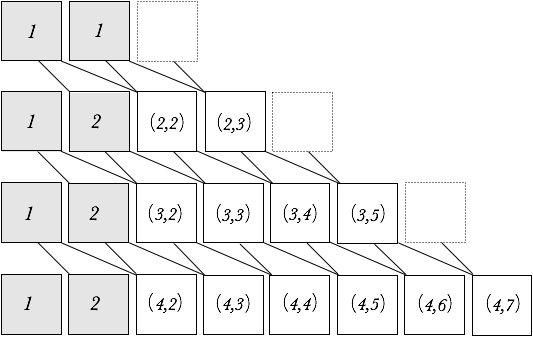
\includegraphics[scale=0.4]{FiguresMaths/TreeProfile}
        \caption{Graphical construction of the triangle profile numbers.}
        \label{Fig:treeprofile}
\end{center}
\end{figure}



%%%%%%%%%%%%%%%%%%%%%%%%%%%%%%%%%%%

\section{Graphs}

\subsection{Spanning Trees}
\label{Appendix:spanningTrees}

Recall here the problem
\bigskip

There are mainly two ways for constructing such a MST, each one
emphasizes a different propriety of the MST, namely, avoid cycles and
minimize the span.  In both cases, the edges are sorted in increasing
order of weights.  More precisely, the first one constructs a subtree
which partially spans the graph by adding at each step the minimum
neighboring edge while the other add successively the edges of minimal
weights that do not create a cycle.

\subsection{Hamiltonian and Eulerian in de Bruijn}
\label{Appendix:hamiltonianDeBruijn}

\noindent {\bf (1)}
%
For any directed graph $\g$, the {\it line digraph} \index{line graph}
\index{line digraph} of $\g$, denoted $\Lambda(\g)$, is the following
directed graph.
\begin{itemize}
\item
The nodes of $\Lambda(\g)$ are the arcs of $\g$:
\[ \n_{{\Lambda}({\cal G})} \ = \ \a_{\fg} \]
\item
For each pair of arcs of $\g$ of the form
\[ \big[a_{x,y} = (x \ \rightarrow \ y) \big] \ \ \ \mbox{ and } \ \ \ 
\big[a_{y,z} = (y \ \rightarrow \ z) \big]
\]
i.e, arcs such that the endpoint of the first arc is the source of the
second arc, $\Lambda(\g)$ contains an arc $(a_{x,y} \ \rightarrow
\ a_{y,z})$.
\end{itemize}
The relevance of this topic to this section is that the line graph of
every de Bruijn network $\d_n$ is the ``next bigger'' de Bruijn
network, $\d_{n+1}$.  Let us verify this claim.

\begin{prop}
\label{thm:deBruin-linegraph}
For all $n \in \N^+$,
$\d_{n+1}$ is the line digraph of $\d_n$: $\d_{n+1} \ = \ \Lambda(\d_n)$.
\end{prop}

\begin{proof}
Each node of $\Lambda(\d_n)$ is an arc of $\d_n$, hence has the form
\[ (\beta x \ \rightarrow \ x \gamma) \]
for $x$ a length-$(n-1)$ binary string and $\beta, \gamma \in
\{0,1\}$.  Let us associate node $\beta x \gamma$ of $\d_{n+1}$ with
this node of $\Lambda(\d_n)$.

\smallskip

Note first that each arc of $\d_{n+1}$ has the form
\[ (\delta y \varepsilon \ \rightarrow \ y \varepsilon \varphi), \]
where $y$ is a length-$(n-2)$ binary string and $\delta, \varepsilon,
\varphi \in \{0,1\}$.  By our association of nodes of $\d_{n+1}$ with
arcs of $\d_n$, this arc of $\d_{n+1}$ does, indeed, correspond to two
successive arcs of $\d_n$.   The first of these successive arcs
{\em enters} node $y \varepsilon$ of $\d_n$; the second {\em leaves}
that node.

Note next that, given any two successive arcs of $\d_n$, say
\[
(\rho \sigma z \ \rightarrow \ \sigma z \tau) \ \ \ \mbox { and } \ \ \
(\sigma z \tau \ \rightarrow \  z \tau \xi)
\]
where $z$ is a length-$(n-2)$ binary string and $\rho, \sigma, \tau,
\xi \in \{0,1\}$, there is, indeed, an arc of $\d_{n+1}$ of the form
\[ (\rho \sigma z \tau \ \rightarrow \ \sigma z \tau \xi) \]
This means that the digraph $\d_{n+1}$ is identical to the digraph
$\Lambda(\d_n)$, modulo a renaming of nodes and arcs.\footnote{Technically,
  we are asserting that the digraphs ${\cal D}_{n+1}$ and ${\Lambda}({\cal D}_n)$ 
  are {\it isomorphic} to one another.  The topic of
  graph isomorphism is beyond the scope of this text, but our informal
  description provides all the details one would need to formalize the
  described isomorphism.}

The described correspondence between the nodes and arcs of $\d_{n+1}$
and $\Lambda(\d_n)$ completes the proof.  \qed
\end{proof}

\begin{figure}[hbt]
\begin{center}
       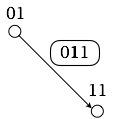
\includegraphics[scale=0.6]{FiguresGraph/dBlabelEdge}
\caption{Illustrating how to label each arc of a de Bruijn network by
  concatenating the labels of the nodes incident to the arc and
  compacting the common intermediate bits.  In the depicted example,
  the node-labels $01$ and $11$ combine to yield the arc-label $011$.}
  \label{fig:dBlabelEdge}
\end{center}
\end{figure}

\medskip

\noindent {\bf (2)}
{\it Eulerian cycles (or tours)}. \index{Eulerian cycle}
\index{Eulerian tour} A {\it directed Eulerian cycle} in a digraph
$\g$ is a directed cycle that contains each arc of $\g$ precisely
once.  We will see, later in this chapter, a truly elementary
argument, based on node-degrees, which proves that every de Bruijn
digraph has a directed Eulerian cycle.  This demonstration will
combine with Proposition~\ref{thm:deBruin-linegraph} to complete the
proof of Proposition~\ref{thm:deBruijn-Hamiltonian}.  \qed
%\end{proof}


\subsection{Coloring a planar graph with 5-colors}
\label{Appendix:5colors}

\begin{prop}[The $5$-Color Theorem for Planar Graphs \cite{Heawood90}]
\label{thm:P-5-colorability}
Every planar graph is $5$-colorable.
\end{prop}


\begin{proof}
The proof combines a sophisticated analysis of the structure of the
planar graph we wish to color with an induction that can be converted
into an efficient algorithm actually achieving the $5$-coloring.

\smallskip

For brevity, let us henceforth discuss only {\em valid} colorings,
i.e., colorings of a graph's nodes in which neighboring nodes get
different colors.

\smallskip

\noindent {\em Base of our induction.}
Because the $5$-clique $\k_5$ is obviously $5$-colorable, so also must
be all graphs having $\leq 5$ nodes.  Therefore, we know that any
non-$5$-colorable graph would have $\geq 6$ nodes.

\smallskip

\noindent {\em Inductive hypothesis.}
Assume, for induction, that every planar graph having $\leq n$ nodes
is $5$-colorable.

\smallskip

\noindent {\em Inductive extension.}
If the proposition were false, then there would exist a planar graph
$\g$ having $n+1$ nodes which is not $5$-colorable.  By
Lemma~\ref{thm:PlanarGraph-degree5}, $\g$ would have a node $v$ of
degree $\leq 5$.  The remainder of the proof focuses on the graph
$\g$, its minimal-degree node $v$, and on $v$'s $(d_v \leq 5)$
neighbors in $\g$.

Now, if there were a coloring of $\g$'s nodes in which $\leq 4$ colors
were used to color $v$'s neighbors, then the following analogue of the
coloring strategy of Proposition~\ref{thm:P-6-colorability} would
produce a $5$-coloring of $\g$.
\begin{enumerate}
\item
Remove node $v$ and its incident edges from $\g$, thereby producing
the $n$-node planar graph $\g'$.
\item
Produce a $5$-coloring of $\g'$ that uses only $4$ colors for the
nodes that are neighbors of $v$ in $\g$.
\item
($a$) Reattach node $v$ and its edges to $\g'$, thereby reconstituting
  $\g$.  ($b$) Color $v$ with whichever of the $5$ available colors is
  not used to color $v$'s neighbors.
\end{enumerate}

In order to proceed in pursuit of a contradiction, we must understand
what structural features of $\g$ make it impossible to use only $4$
colors on $v$'s neighbors when $5$-coloring $\g$.  There are three
important situations to recognize.
\begin{description}
\item[{\sf Case 1}.]
Node $v$ has degree $\leq 4$.

\smallskip

By definition, $\leq 4$ colors are used to color $v$'s neighbors in
this case.
\end{description}
Note that, in all remaining cases, node $v$ has precisely $5$
neighbors---or else, we would have invoked Case 1 to color $\g$ with
$5$ colors.
\begin{description}
\item[{\sf Case 2}.]
For some $5$-coloring of $\g$, $\geq 2$ neighbors of $v$ get the same
color.

\smallskip

Because $v$ has exactly $5$ neighbors, in this case, only $4$ colors
are used to color these neighbors.
\end{description}
In all remaining cases, the $5$ neighbors of $v$ receive distinct
colors.
\begin{description}
\item[{\sf Case 3}.]
For some $5$-coloring of $\g$, some two neighbors of $v$, call them
$v_1$ and $v_2$, reside in distinct components of $\g$ once $v$ and
its incident edges are removed from $\g$.

\smallskip

As before, let $\g'$ be the (in this case, disconnected) graph that
results when $v$ and its incident edges are removed from $\g$.  For $i
= 1,2$ Let $\g_i$ be the component of $\g'$ that contains node $v_i$.

Say that, under the $5$-coloring of $\g$ that we are focusing on,
$v_1$ is colored {\it red} and $v_2$ is colored {\it green}.

Let us recolor the nodes of $\g_1$ so that node $v_1$ is now colored
{\it green}.  (One needs only switch the colors {\it red} and {\it
  green} in the existing coloring of $\g_1$.)  It is always possible
to do this in a way that does not affect the valid coloring of $\g_2$
because $\g_1$ and $\g_2$ are mutually disjoint.

Once we have thus-recolored $\g_1$, we have a $5$-coloring of $\g$ for
which Case 2 holds.  (In fact, we can color node $v$ {\em red} when we
reattach it to $\g'$.)
\end{description}

\noindent
We now see that Cases 1--3 cannot prevent us from $5$-coloring $\g$, so
we are left with the following minimally constrained situation.
\begin{description}
\item[{\sf Case 4}.]
\begin{itemize}
\item
Every minimum-degree node of $\g$ has $5$ neighbors.

For the minimum-degree node $v$, let us call these neighbors $v_1$,
$v_2$, $v_3$, $v_4$, $v_5$, in clockwise order within the planar
drawing.
\item
In every $5$-coloring of $\g$, the neighbors of every minimum-degree
node receive distinct colors.

For node $v$, let us say that neighbor $v_i$ receives color $c_i$.
\end{itemize}
{\Denis Check carefully the ref to the figures...}

\begin{figure}[hbt]
\begin{center}
       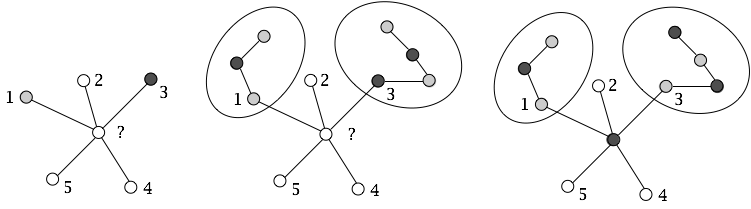
\includegraphics[scale=0.4]{FiguresGraph/5colorsCase1}
\caption{to be completed}
  \label{fig:5colorsCase1}
\end{center}
\end{figure}
The leftmost graph in Fig.~\ref{fig:5colorsCase1} depicts the portion of $\g$ comprising
node $v$ and its neighbors.  In the figure, we use integer $i$ to
denote, ambiguously, node $v_i$ and its assigned color $c_i$.  The
question mark ``?'' that ``colors'' node $v$ indicates that we do not
yet know what color to assign to $v$.  The other two graphs in the
figure depict schematically how we have dealt with Case 3 above.
{\Denis Clarify which are the concerned graphs here}
\begin{itemize}
\item
All neighbors of node $v$ remain in the same component of $\g$ when
$v$ and its incident edges are removed.
\end{itemize}
\end{description}
To analyze Case 4, we focus on nodes $v_1$ and $v_3$ in Fig.~\ref{fig:5colorsCase2}.
Importantly, these nodes have received distinct colors ($c_1$ and $c_3
\neq c_1$, respectively), and these nodes are not adjacent to one
another as one makes a clockwise sweep around node $v$.
\begin{figure}[hbt]
\begin{center}
       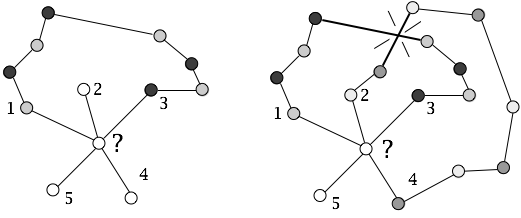
\includegraphics[scale=0.4]{FiguresGraph/5colorsCase2}
\caption{{\Denis to be completed}}
  \label{fig:5colorsCase2}
\end{center}
\end{figure}

Now take $\g$ and focus only on the nodes that are colored $c_1$ or
$c_3$ (as are $v_1$ and $v_3$, respectively) and on the nodes that are
colored $c_2$ or $c_4$ (as are $v_2$ and $v_4$, respectively).  One
sees from Fig.~\ref{fig:5colorsCase2} that:
\begin{itemize}
\item
$\g$ can, {\em but need not}, contain a path whose nodes alternate
  colors $c_1$ and $c_3$---call this a ``$c_1$-$c_3$ path'' between
  nodes $v_1$ and $v_3$.
\item
$\g$ can, {\em but need not}, contain a path whose nodes alternate
  colors $c_2$ and $c_4$---call this a ``$c_2$-$c_4$ path'' between
  nodes $v_2$ and $v_4$.
\item
$\g$ {\em cannot} contain both of the paths just described, i.e., a
  $c_1$-$c_3$ path between $v_1$ and $v_3$ {\em and} a $c_2$-$c_4$ path
  between $v_2$ and $v_4$.

{\em These two paths, if they existed, would cross one another---which
  is forbidden because $\g$ is a {\em planar} graph.}  See Figure 2.
\end{itemize}
It follows that {\em either} $\g$ does not contain a $c_1$-$c_3$ path
between $v_1$ and $v_3$ {\em or} $\g$ does not contain a $c_2$-$c_4$
path between $v_2$ and $v_4$.  Say, with no loss of generality, that
the former path does not exist.  Then we can switch colors $c_1$ and
$c_3$ beginning with node $v_1$ and obtain a coloring of $\g$ in which
$v_1$ and $v_3$ both receive the color $c_3$.  We can then proceed as
in Case 2 to get a $5$-coloring of $\g$.

This four-case analysis shows that we can always produce a
$5$-coloring of $\g$, which completes the proof.  \qed
\end{proof}

